\section{Results/Numerical Experiments}
In the following, we first look at groups of constraints individually and conduct experiments to show their impact. Then we look at results for a full-scale, realistic network of port calls and perform some scaling experiments. %An illustration of the key number that our model can show, is illustrated for a small network in the appendix. 

For all of the following experiments, $L=\{20,40\}$ and $W = \{5,13,19,26\}$, and $T=L\times W\times \{\text{R},\text{NR}\}$ is the set of considered types of a container group. We use a vessel with 23 bays, and we {divide the vessel in up to 26 sections (i.e., $|S| = 26$ )} each spanning one or zero bays. The sections that cannot contain cargo are included to improve precision of hydrostatic constraints. Non-ballast tanks are assumed filled 70\%.

In the experiments, we compare with a so-called simple model, which is a vessel capacity model that takes into account the total TEU capacity, the total reefer capacity, and the total displacement (corresponding to the constraints \eqref{capTEU}, \eqref{caprc}, and \eqref{capDisp} for the single section including the whole vessel).


\subsection{Vessel constraints} % (single-ship optimizations)
Our first series of experiments look at the vessel constraints separately, i.e. we consider the constraints defining $\mathit{SCM}^\ttt{v}_{e}$ in \eqref{sailingCon} for a single sailing edge $e$. 
For all experiments in this section, $|S| = 26$.
Since we only consider a single vessel in these experiments, we do not consider all the properties of container groups (e.g., the destination port is irrelevant). Thus, in the following experiments, we only refer to the type of a container group, i.e. the length, the weight class and whether it is a reefer container or not. 

\subsubsection{Vessel capacity constraints and hydrostatic constraints}
To investigate the impact of the vessel capacity constraints (constraints \eqref{cap20}-\eqref{capDisp}), we find the maximal number of containers of a type $t\in T$ that can be placed on a vessel with a given ROB cargo. This number is found in the case where all vessel capacity constraints are enforced, and in the case when only 3 basic constraints capcity are considered are enforced (the simple model described above).
The ROB cargo is constructed with heavy cargo in the fore- and aft-most horizontal sections while it is empty in the middle horizontal sections. It is given in Table~\ref{tab:ROBCap} and shows the number of each type of container in non-empty bays, on and below deck.

\begin{table}[width=.9\linewidth,cols=11,pos=h]
\caption{ROB cargo for experiment with vessel capacity constraints and hydrostatic constraints.}\label{tab:ROBCap}
\begin{tabular*}{\tblwidth}{@{} R *{10}C @{}}
\toprule
&\multicolumn{10}{c}{Bay (on deck-below deck)}\\
\cmidrule{2-11}
Container type&1&2&3&4&5&19&20&21&22&23\\
\midrule
40', 26t, NR &  70-28 & 105-60 & 80-100& 90-115& 90-135& 72-0 & 42-132 & 42-110 & 33-92 & 33-24\\

\bottomrule
\end{tabular*}
\end{table}

The results of the optimizations are given in Table~\ref{tab:resultsCap}, where also the overestimation (O.e.) is shown given in percentage of the more constrained model. 
\\\\
To investigate the effects of the hydrostatic constraints, we have made two similar experiments. First we use a model with vessel capacity constraints and hydrostatic constraints (constraints \eqref{cap20}-\eqref{draftLimits}), where ballast tanks can be filled freely within the upper limits. Again we optimize the number of containers of each type that can be placed on the vessel with the given ROB. Afterward, the optimizations are repeated where we further require that the tanks are left empty, which might be a reasonable requirement on long legs in order to prevent wear and tear.
 
The results are shown in Table~\ref{tab:resultsCap} as  well as the overestimation (O.e.) of a model compared to a more constrained model. This overestimation is given in percentage of the objective value of the more constrained model and is shown in a column between the two models being compared.

%
\begin{table}[width=.95\linewidth,cols=10,pos=h]
\caption{Maximal number of containers of each type that can be placed on the vessel, when vessel capacity constraints and hydrostatic constraints are/are not included, respectively. The columns marked ``O.e.'' indicates the overestimation between the two models on either sides. }\label{tab:resultsCap}
\begin{tabular*}{\tblwidth}{@{} r@{\hskip3pt}r@{\hskip3pt}r *{7}{R} @{}}
\toprule
&&&\mult{7}{c}{Included constraints}\\
\cmidrule{4-10}
	&	 &	&		 &		&		   &		&Capacities,  &		  &Capacities,\\		
	&	 &	& 		 &		&Capacities&		&hydrostatics,&	    &hydrostatics,\\	
\mult{3}{c}{Type}
				     &	Simple &O.e.   &(No tanks)&O.e.&tanks free   &O.e. &tanks empty	\\		
\midrule
20',& 5t,&NR& 12802.0& 14.8 & 11151.6  & 6.7& 10450.1 		& 19.4&  8751.3\\
20',& 5t,& R&  2024.0& 31.3 &  1542.0  & 0.0&  1542.0 		&  0.0&  1542.0\\
20',&13t,&NR&  7900.9& 0    &  7900.9  & 3.2&  7658.3 		&  0.0&  7658.3\\
20',&13t,& R&  2024.0& 31.3 &  1542.0  & 0.0&  1542.0 		&  0.0&  1542.0\\
20',&19t,&NR&  5405.9& 0    &  5405.9  & 1.6&  5322.3 		&  0.1&  5319.0\\
20',&19t,& R&  2024.0& 33.0 &  1522.2  & 1.6&  1498.6 		&  0.0&  1498.6\\
20',&26t,&NR&  3950.5& 0    &  3950.5  & 1.6&  3889.4 		&  0.1&  3887.0\\
20',&26t,& R&  2024.0& 53.5 &  1318.3  & 1.8&  1295.5 		&  0.0&  1295.5\\
40',& 5t,&NR&  6401.0& 0.3  &  6379.0  &15.7&  5513.1 		& 19.6&  4608.6\\
40',& 5t,& R&  2024.0& 118.8&   925.0  & 0.0&   925.0 		&  0.0&   925.0\\
40',&13t,&NR&  6401.0& 2.3  &  6255.0  & 9.5&  5713.8 		& 14.6&  4985.7\\
40',&13t,& R&  2024.0& 118.8&   925.0  & 0.0&   925.0 		&  0.0&   925.0\\
40',&19t,&NR&  5405.9& 0    &  5405.9  & 4.1&  5191.6 		&  2.4&  5069.5\\
40',&19t,& R&  2024.0& 118.8&   925.0  & 0.0&   925.0 		&  0.0&   925.0\\
40',&26t,&NR&  3950.5& 0    &  3950.5  & 0.0&  3950.5 		&  0.0&  3950.5\\
40',&26t,& R&  2024.0& 121.0&   915.7  & 0.0&   915.7 		&  0.0&   915.7\\
\bottomrule
\end{tabular*}
\end{table}

Clearly, using all vessel capacity constraints already makes a large difference compared to only using the simple model's constraints. For this example, this is particularly true for reefer containers. For 40' containers, this results in an overestimation of more than 100\%, while it is between app. 30-50 \% for 20' reefers. We remark that this is not only caused by non-reefer ROB cargo taking up reefer capacity, since only one bay containing ROB have reefer capacity, while there is free reefer-capacity in 6 other bays (in total 1760 TEU (87\% of the total reefer capacity)).  Additionally, for light 20' non-reefers, the overestimation is 14.8\%.
%[I assume that this is mainly because of weight-capacities of bays and of course that ROB is placed at specific places.]%[It is only bay 5 in which ROB takes up reefer capacity, however, reefers can apparently not just be placed in the corresponding slots, probably (?) due to weight capacity.]

Looking at the results for the hydrostatic constraints, we see that the number of containers that are possible to load differs for several types of containers. Most noticeable, for 40' non-reefer containers with a weight of 5t, the overestimation that the model only including vessel capacities does, compared to the model with additional hydrostatic constraints (but free containers) is 15.7\%, while that number is 9.5\% for 40' non-reefer containers with a weight of 13t, and 6.7\% for 20' non-reefer containers of 5t. If it is further required that the ballast tanks should be empty, we get an overestimation (compared to the model where hydrostatic constraints are included, but the tanks can be filled) of 19.6\% for 40' non-reefers of 5t, 19.4 \% for 20' non-reefers of 5t, and 14.6 \% for 40' non-reefers of 13t.

\subsubsection{GM and lashing constraints}
For testing the impact of the GM-constraints (constraints \eqref{defGM}-\eqref{positiveLambdas}), a vessel have been filled with light ROB cargo \emph{below} deck as given in Table~\ref{tab:ROBGM}. The table shows the number of the given type of container in all bays below deck; there is no cargo above deck.\\

\begin{table}[width=.9\linewidth,cols=13,pos=h]
\caption{ROB cargo for experiment with GM constraints. There is no cargo below deck.}\label{tab:ROBGM}
\begin{tabular*}{\tblwidth}{@{}*{13}{R}@{}}
\toprule
&\multicolumn{12}{c}{Bay (on deck)}\\
\cmidrule{2-13}
Container type&1&2&3&4&5&6&7&8&9&10&11&12\\
\midrule
40', 5t, NR & 35&68&96&116&134&152&170&182&194&204&208&212\\
\multicolumn{5}{c}{}\\
&&13&14&15&16&17&18&19&20&21&22&23\\
\cmidrule{3-13}
40', 5t, NR &&210&161&202&188&184&160&142&128&106&88&20\\
\bottomrule
\end{tabular*}
\end{table}

For the first GM-experiment, we then require that nothing is put above deck in bays other than bay 12, and we optimize intake of each container group individually, in bay 12 above deck. Capacity constraints and hydrostatic constraints are included, and the tanks can be filled as needed (requiring tanks to be empty does not influence the results in this case). We only allow containers of the type in question on board. %, afterwards, other types are also allowed in order to fit more on board.
%When only one type is allowed on board we get a bit different result for non-reefers of 5 or 13 t; (20,5: 316.1), (20,13: 257.9), (40,5: 195.3), (40,13: 176.4). This also gives difference on 24%, 6.3 %, 0.2%, 11.1%). Also different numbers (a little) in +GM+t=0, in the columns where GM is included, where the numbers are between 0.2 and 2.3 lower. Also, in this case the hydrostatics don't add to the result - for plain capacities, the numbers are the same as in the first column]. 

The results are shown in Table~\ref{tab:resultsGM}. The table only shows the results for the types for which the inclusion of the GM constraint makes a difference in the result.
%Plain capacities gives same result as first column
\begin{table}[width=.9\linewidth,cols=6,pos=h]
\caption{Maximal number of containers of each type that can be stowed above deck in bay 12.}% (when no other types are allowed).}
\begin{tabular*}{\tblwidth}{@{} r@{\hskip3pt}r@{\hskip3pt}r@{} RRR@{}}
\toprule
\multicolumn{3}{l}{Container type}
			&Without GM		&With GM		&Overestimation (\%)\\%With GM, other types allowed too & Overestimation (\%)\\		
\midrule
\quad\quad	20',& 5t,&NR&    392.0  	&     316.1 	&24.0\\%&  368.0\\%6.5%& 24.0\\ % +0.4
			20',&13t,&NR&    274.2  	&     257.9 	& 6.3\\%&  265.0\\%&3.5% 6.3\\ % +2.3
			40',& 5t,&NR&    196.0  	&     195.3 	& 0.4\\%&  196.0\\%&0 0.2\\ % +0.2
			40',&13t,&NR&    196.0  	&     176.4 	&11.1\\%&  188.1\\%&4.2% 11.1\\
			40',&19t,&NR&    167.9  	&     165.1 	& 1.7\\%&  165.1\\%& 1.7\\
\bottomrule
\end{tabular*}
\label{tab:resultsGM}
\end{table}

The results show that without GM constraints, the model overestimates the number of containers that can fit on that particular bay above deck for 5 types of containers. The overestimation is most noticeable in the case of 20' non-reefers of 5t (24.0\%), 40' non-reefer of 13t (11.1\%), and 20' non-reefers of 13t (6.3\%).
\\\\
In the second GM-experiment we optimize cargo over the whole vessel, with and without GM-constraints. %, and with and without requiring that ballast tanks should be empty.
Again, vessel capacity and hydrostatic constraints are included. We optimize the number of containers of a given type that can be loaded to the vessel.
The results are shown in Table~\ref{tab:resultsGM2}. Only types for which there is a difference in objective value for the looked-at models are included.
%Caps alone same as first column
%reefer-results left out; they are the same across the board. The capacities at the different locations are already so small, that gm won't matter in these cases. Although, maybe, if we could have more onboard thna just that one type (ie. is it possible to bring something else as well, it might make a difference. Hm, it seems to be the same thing. Did I make a mistake?

\begin{table}[width=.9\linewidth,cols=9,pos=h]
\caption{Results when optimizing number of containers of each type with and without GM constraints. O.e. stands for overestimation.}% in percentage of the objective of the most constraining model.}
\label{tab:resultsGM2}
\begin{tabular*}{\tblwidth}{@{} r@{\hskip3pt}r@{\hskip3pt}r*{6}R @{}}%|*{5}{r}}
\toprule
&&&\mult{6}{c}{Included constraints}\\
\cmidrule{4-9}
%&&&\mult{6}{c|}{Tanks free}&\mult{5}{c}{Tanks empty}\\
&&&\mult{3}{c}{All types allowed}&\mult{3}{c}{Only 1 type}\\%&\mult{3}{c}{All types allowed}&\mult{2}{c}{Only 1 type}\\
\cmidrule{4-6} \cmidrule{7-9}
\multicolumn{3}{c}{Type}					                                               						
				  	&	 - GM  		& + GM		&O.e.				& -	GM		  &	+ GM		&O.e.			\\%& - GM	 			 & + GM	    &O.e.		  & - GM 			& + GM	 \\		
\midrule																																					
20',& 5t,&NR&   7549.6 	&  6585.0 & 14.6			&	7549.6	  & 6453.1	& 17.0  	\\%&  7549.6 		 &  6567.3	& 15.0 		&	6447.3		&  6447.3\\	 
20',&13t,&NR&   4870.6 	&  4661.3 &  4.5			&	4860.0	  & 4521.0  &  7.5  	\\%&  4789.9 		 &  4553.8	&  5.2 		&	4259.3		&  4259.3\\
20',&19t,&NR&   3387.5 	&  3384.8 &  0.1			&	3384.9	  & 3373.2  &  0.3  	\\%&  3327.7 		 &  3241.2	&  2.7 		&	3111.1		&  3111.1\\
20',&26t,&NR&   2522.3 	&  2522.3 &	 0.0			&	2520.8	  & 2510.9  &  0.4  	\\%&  2474.8 		 &  2411.7	&  2.6 		&	2327.0		&  2327.0\\ 
40',& 5t,&NR&   7854.0 	&  7838.7 &  0.2			&	7854.0	  & 7838.7  &  0.2  	\\%&  7854.0 		 &  7834.7	&  0.2 		&	7834.7		&  7834.7\\ 
40',&13t,&NR&   4494.0 	&  4054.4 & 10.9			&	4494.0	  & 4054.4  & 10.9  	\\%&  4416.7 		 &  3998.8	& 10.5 		&	3992.9		&  3992.9\\ 
40',&19t,&NR&   3930.5 	&  3801.5 &  3.4			&	3930.5	  & 3801.5  &  3.4  	\\%&  3760.4 		 &  3684.8	&  2.1 		&	3684.8		&  3684.8\\ 
40',&26t,&NR&   2897.8 	&  2894.1 &  0.1			&	2897.8	  & 2894.1  &  0.1  	\\%&  2769.4 		 &  2736.3	&  1.2 		&	2736.3		&  2736.3\\ 
\bottomrule
\end{tabular*}
\end{table}
\red{I also have result for when tanks are required empty, but that is a bit too much, I think, though the results/differences are a bit higher}%{[Note to self: Is it the right results I copied for the empty tanks, all types - there is no difference]}

As can be see from the results in Table~\ref{tab:resultsGM2}, including GM constraints can have a big impact on the number of containers of a given type that can be loaded on the vessel. Most noticeable, depending on whether or not we only allow the container type in question to be loaded or not, %and whether the tanks are required to be empty or not, 
the overestimation is between 14.6 and 17.0\% for 5t 20' non-reefers. Likewise, the overestimation for 40' non-reefers of 13t is %between 10.5 and 
10.9\%, and it is between 4.5 and 7.5\% for 20' non-reefers of 13t. %This holds unless only that particular type can be loaded and tanks are required to be empty, in which case there is no difference in all the given instances [check it].

\subsection{Terminal constraints} %(Single-service, multi-port optimizations)
In the following series of experiments, we will look at the terminal constraint (summarized in \eqref{terminalCon}) separately. We use the same vessel and the same sectioning as in the previous experiments.  

To show the potential impact of the different terminal constraints, we consider the very simple network consisting of the 3 port calls made by the same vessel: $\mathfrak{A} \rightarrow \mathfrak{B} \rightarrow \mathfrak{C}$. The ports of the port calls are assumed to be different, and the dates of the port calls are assumed to come in the given order. Besides these properties, we do not care about (and hence do not mention) the particular ports, dates (and vessel) of the port calls, and likewise we leave out mention of yard-side and vessel-side nodes. 

\subsubsection{Overstowage}
For investigating the effect of the overstowage constraints (constraint \eqref{overst}), we look at a vessel with the ROB cargo given in Table~\ref{tab:ROBOverst}. The vessel contains in total 4977 containers - mainly on deck - to be delivered (discharged) at the last port call $\mathfrak{C}$, and we require that 2000 containers (40' non-reefers of 19t) destined for the second port call $\mathfrak{B}$ needs to be loaded at the first port call $\mathfrak{A}$. The minimal needed moves to handle the ROB cargo and the exported cargo (loading and unloading) in this situation is therefore $4977 + 2\cdot 2000 = 8977$ moves.%; this is the case whether or not hydrostatic and gm constraints are included or not.  

\begin{table}[width=.9\linewidth,cols=17,pos=h]
\caption{ROB cargo for overstowage experiment.}\label{tab:ROBOverst}
\begin{tabular*}{\tblwidth}{@{} R *{8}C @{}}
\toprule
&\multicolumn{8}{c}{Bays (on deck - below deck)}\\
\cmidrule{2-9}
Container group&1&2&3&4&5&6&7&8\\
\midrule
40',13t,NR $\rightarrow \mathfrak{C}$
					& 110-11 & 129-22 & 144-30 & 157-36  & 157-42 & 157-47 & 157-52 & 157-56\\
\multicolumn{5}{c}{}\\
&9&10&11&12&13&14&15&16\\
\cmidrule{2-9}
40',13t,NR $\rightarrow \mathfrak{C}$
					& 157-59 & 157-62	& 157-64 & 157-216 &157-210 & 157-50 & 157-62	& 157-58\\
\multicolumn{5}{c}{}\\
&&17&18&19&20&21&22&23\\
\cmidrule{3-9}
40',13t,NR $\rightarrow \mathfrak{C}$
					&& 157-57 & 157-49 & 157-44 & 157-105 & 157-88 & 157-27 & 157-7\\
\bottomrule
\end{tabular*}
\end{table}

We now look at the minimal number of moves required in a number of scenarios where different constraints are included, i.e. the objective function is a minimization of these moves. All scenarios include the overstowage constraint. First we only additionally include vessel capacity constraints, then we further add hydrostatic constraints, and then further GM constraints. %Table~\ref{tab:resultsOverst} summarizes the required moves for loading/unloading cargo, when overstowage is considered, in a case where the cargo being moved is forced back to where is was removed from (same section), and in a case where this is not required (i.e. it can be freely repositioned as our model is presented). 
For each scenario, we consider a case where cargo can be freely restowed, and a case where cargo is forced to be placed in the section from which is was removed.
Table~\ref{tab:resultsOverst} summarizes the results. %required moves for loading/unloading cargo, when overstowage is considered, in a case where the cargo being moved is forced back to where is was removed from (same section), and in a case where this is not required (i.e. it can be freely repositioned as our model is presented).

\begin{table}[width=.9\linewidth,cols=5,pos=h]
\caption{Required moves and underestimation of moves when different sets of constraints are included.}\label{tab:resultsOverst}
\begin{tabular*}{\tblwidth}{@{} LRRRR@{}}
\toprule
& \mult{4}{c}{Required moves}\\
\cmidrule{2-5}
Model/Included constraints	& + Repo. & U.e. (moves / \%) & - Repo. & U.e. (moves / \%)\\
\midrule
Simple 						& 8977    & - 			  & 8977 	&  - \\
Capa., overst				& 10969.4 & 1992.4 / 18.2 & 9973.2 	&  996.2 / 10.0\\
Capa., hydro., overst.		& 10969.4 & 1992.4 / 18.2 & 9973.2 	&  996.2 / 10.0\\
Capa., hydro., GM, overst. 	& 12531.0 & 3554.0 / 28.4 & 10810.7 & 1833.7 / 17.0\\
\bottomrule
\end{tabular*}
\end{table}

As the results show, not including these overstowage constraints can lead to a considerable underestimation of the number of required moves (17.0 or 28.4\% depending on whether or not containers can be freely repositioned after being moved due to overstowage).

\subsubsection{Cranes and port stay}
As before, we consider the network $\mathfrak{A} \rightarrow \mathfrak{B} \rightarrow \mathfrak{C}$. On board the vessel is ROB cargo to $\mathfrak{C}$ and $\mathfrak{A}$, respectively, as shown in Table~\ref{tab:ROBPS}. 
The table shows the number of each type of container in each non-empty bay, on and below deck. As the ROB cargo shows, 300 containers need to be discharged (imported) at port call $\mathfrak{A}$, and all this cargo is placed in one bay only.

\begin{table}[width=.9\linewidth,cols=9,pos=h]
\caption{ROB cargo for experiments with cranes and port stay.}\label{tab:ROBPS}
\begin{tabular*}{\tblwidth}{@{} R *{8}C @{}}
\toprule
&\mult{8}{c}{Bay (on deck - below deck)}\\
\cmidrule{2-9}
Container type&1&2&3&7&8&10&13&14\\
\midrule
40',13t,NR $\rightarrow \mathfrak{C}$&  -12 & 36-30 & 66-78 & 150-174 & 150-186 &    -    & 150-214 & 150-165\\
40',13t,NR $\rightarrow \mathfrak{A}$&  -   &   -   &   -   &    -    &    -    & 150-150 &    -    &    -   \\
\mult{5}{c}{}\\
&&15&18&19&20&21&22&23\\
\cmidrule{3-9}
40',13t,NR $\rightarrow \mathfrak{C}$&& 150-206 & 44-40 & 44-66 & 88-92 & 132-90 & 132-92 & 132-24\\
40',13t,NR $\rightarrow \mathfrak{A}$&&    -    &   -   &   -   &   -   &    -   &    -   &    -\\
\bottomrule
\end{tabular*}
\end{table}

At port call $\mathfrak{A}$ it is possible to load (export) cargo to port call $\mathfrak{C}$, but only 40' non-reefers of 13t. There is no other export options. In our experiments we then optimize the amount of container of that particular group that can be loaded, when different sets of constraints are included. We start with only including vessel capacity constraints and successively include hydrostatic constraints, GM constraints, overstowage constraint, maximal moves (i.e. constraining the total number of moves at a port, constraint \eqref{minPortStay} combined with \eqref{maxPs}), and then finally the long crane constraints (constraints \eqref{longCrane} and \eqref{longCrane1Bay}). %All models have free tanks.

For this test we let the time window be 20h, and we have 7 cranes at our disposal. If the time window and number of cranes are reduced, the objective value will of course be further reduced, but these values are not unreasonable low. 
The results can be seen in Table~\ref{tab:resultsPS}. 

\begin{table}[width=.9\linewidth,cols=2,pos=h]
\caption{Maximal load/export of 40', 13t non-reefers.}\label{tab:resultsPS}
\begin{threeparttable}
\begin{tabular*}{\tblwidth}{@{} LR @{}}
\toprule
Constraints included						  		&Exported containers\\
\midrule
Capa., 												&4961.0\phantom{\tn{$^{*}$}}\\
Capa., hydro. 										&4961.0\phantom{\tn{$^{*}$}}\\
Capa., hydro., GM									&4627.8\phantom{\tn{$^{*}$}}\\
Capa., hydro., GM, overst.							&4627.8\phantom{\tn{$^{*}$}}\\
Capa., hydro., GM, overst., max. moves:				&3900.0\tn{$^{*}$}\\ 
Capa., hydro., GM, overst., max. moves, long crane:	&3717.6\phantom{\tn{$^{*}$}}\\
\bottomrule
\end{tabular*}
\begin{tablenotes}
\item[$^*$]Using all available crane moves.
\end{tablenotes}
\end{threeparttable}
\end{table}

When including the maximal moves-constraints, we get that the maximal number of containers that can be loaded (*) equals $20\text{ hours}\cdot7\text{ cranes}\cdot 30 \frac{\text{moves}}{\text{hour and crane}} - 300 \text{ moves} = 3900$, i.e. we use all the available crane moves.  
When we further add the long crane constraints, the amount of containers of the given type that can be loaded (exported) is further reduced, because many moves are required to be at the same bay.

%%%%%%%%%%%%%%%%%%%%%%%%%%%%%%%%%%%%%%%%%%%%%%%%%%%%%%%%%%%%%%%%%
\subsection{Small network}\label{sec:smallNetwork}
Before presenting results for a realistically sized network, we will make a demonstration on a much smaller example network, namely the network of port calls made by two vessels shown in Figure~\ref{fig:Network2ServicesB}. As for the previous experiments, the example is constructed to show the impact of the constraints.  
The appendix gives a preview of which information can be extracted from the model, and it also shows ROB cargo and loadlists.
%
%In reality, the network of port calls continues beyond the last date in $\mc{D}$ since the vessels will continuously repeat their cyclic journeys. In order to avoid that our model greedily imports profitable cargo in the later port calls in the network (without regard to how (or if) it will be unloaded later) while simultaneous leaving cargo at the yards, we therefore introduce a \emph{horizon} $H\in\mc{D}$, that indicates the (end of) the time period in which we export cargo. Thus, $\mi{Ex}^{g+}_i=0$ for all yard-side nodes $i$ whose port call is later than $H$. At the same time, it will only be possible to export container groups with a deadline before the last day in $\mc{D}$, thus $\mc{G}=\mc{G}'$. The part of the network after the horizon only serves to empty the vessel, and since e.g. the hydrostatic constraints might not hold for a (half-) empty vessel, the hydrostatic constraints are only enforced for sailing edges before the deadline. In fact, we only enforce network constraints, vessel capacity constraints and the overstowage constraint on edges/port calls after the horizon. 
The horizon is here set to 11.

\begin{figure}
	\begin{center}
		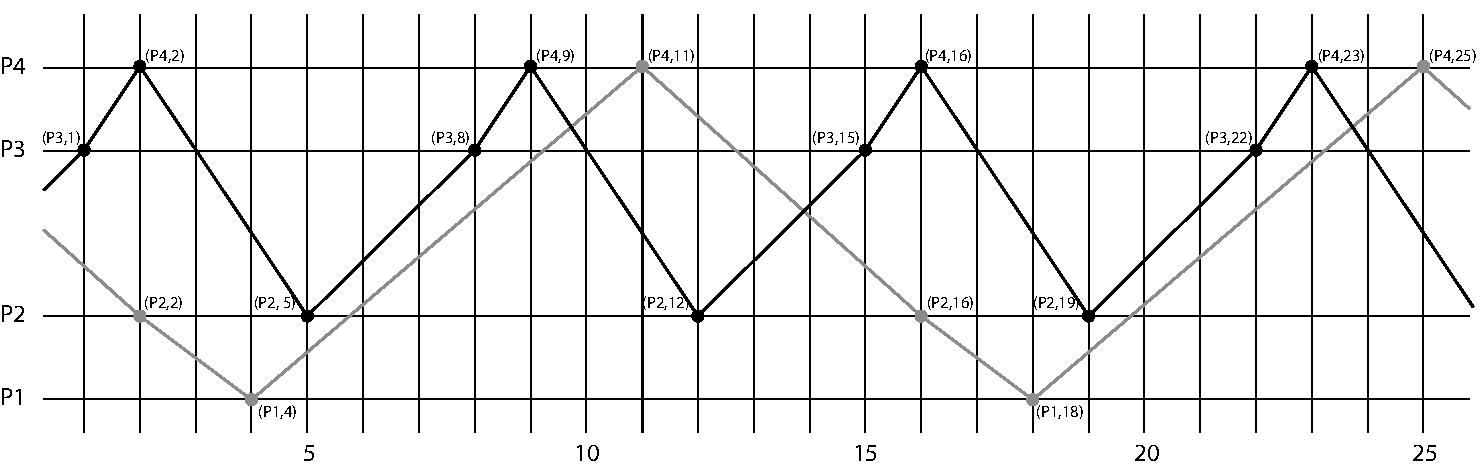
\includegraphics[scale = 0.54]{figures/Network2ServicesB.pdf}
	\caption{Small network of port calls with two services.}
	\label{fig:Network2ServicesB}
	\end{center}
\end{figure}

For this experiment, we use the same type of vessel for both vessels. The used vessel is very large, and this size does not fit well with a small network like the one considered for this experiment. The small number of ports visited by each vessel means that if the vessel is filled adequately then an improbable large amount of time is needed at each port to load and discharge cargo. 
To achieve a more realistic residual capacity, some of the ROB cargo is assumed to be destined to a time and place after the last date and it is not allowed to be left at yard to be picked up later. However, the cargo is allowed to be rearranged.

The vessel is divided into 6 sections. 
\red{Something short about which type of cargo etc? well, I guess also something about the yield (which is otherwise only explained later (?))}
The appendix contains tables showing the content of the vessel (divided into sections) as well as other key values for each of the sailing edges and each of the port calls.

Table~\ref{tab:ObjSmall} shows the objective value (the profit) when considering this network. As in the previous section we have added constraint groups one by one to see the impact of these. The abbreviations in the table is as follows: C: capacity constraints (\eqref{cap20}-\eqref{capDisp}), H: hydrostatic constraints (\eqref{defResF}-\eqref{draftLimits}), GML: GM limits (\eqref{defGM}-\eqref{minGM}), L: lashing constraints (\eqref{convexGM1}-\eqref{positiveLambdas}), O: Overstowage constraint (\eqref{overst}), MM: max moves constraints (\eqref{defMoves}-\eqref{maxPs}), and LC: long crane constraints (\eqref{longCrane}-\eqref{longCrane1Bay}). All experiments include the network flow constraint (\eqref{OnOff}-\eqref{sinks}).

\begin{table}[width=.9\linewidth,cols=2,pos=h]
\caption{Profit for small network with various constraints included}\label{tab:ObjSmall}
\begin{tabular*}{\tblwidth}{@{} LR @{}}
\toprule
						&Profit	(M\$)\\	
\midrule
Simple					&42.94\\	
\midrule                   
C						&30.46\\
C+H						&30.46\\
C+H+GML					&30.15\\
C+H+GML+L	(full $\mi{SCM}^\ttt{v}$)	
						&29.99\\
C+H+GML+L+O				&29.94\\	
C+H+GML+L+O+MM 			&20.75\\
C+H+GML+L+O+MM+LC (full $\mi{SCM}^\ttt{v}$ and full $\mi{SCM}^\ttt{t}$)
						&20.75\\
\bottomrule
\end{tabular*}
\end{table}

\red{Explanation of the results in the table}
%%%%%%%%%%%%%%%%%%%%%%%%%%%%%%%%%%%%%%%%%%%%%%%%%%%%%%%%%%%%%%%%%%
\subsection{Scaling results - Full-scale network}
\begin{figure}
	\centering
		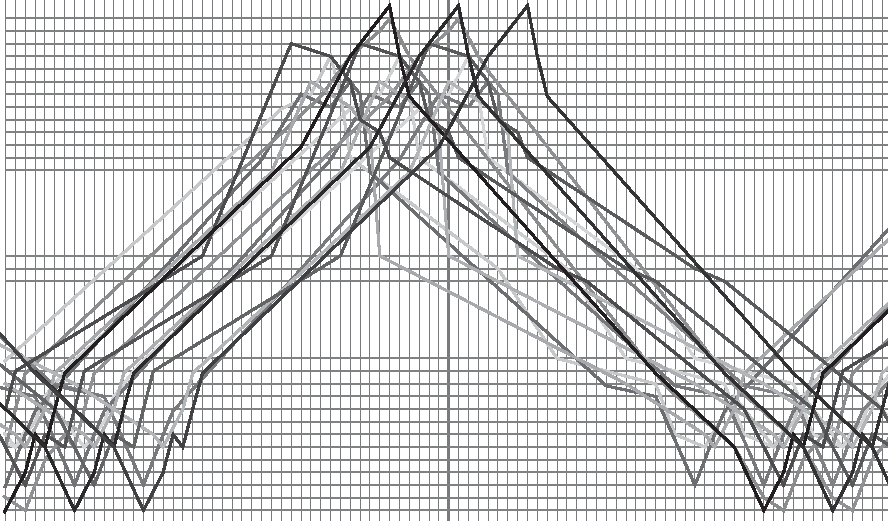
\includegraphics{figures/fewerBW.pdf}
	\caption{Vessels transporting cargo in a network from Asia to Europe within a set period of time.}
	\label{fig:full}
\end{figure}

\noindent To test our model on a full-scale network, we first consider a network of 6 different services, $R_1$ to $R_6$, that are repeated each week, resulting in a network of 67 vessels. The services connect two regions, Asia and Europe, and we are interested in maximizing the flow of cargo from one region to the other in a period of 45 days, which in the considered network is approximately the time it takes for any vessel to get from the first port visited in a region to the first port in the other region. Therefore we restrict our attention to the vessels that in the given time frame of 45 days have port calls first in Asia and then in Europe. This results in the network of $17$ vessels that are shown in Figure~\ref{fig:full}. Each service employ 3 vessel, except for service $R_3$ which only employs 2 vessels.

Each vessel already contain cargo that partly has destinations in Asia (that has not been delivered yet), and cargo with a destination in Europe (exported at the port calls in Asia prior to the current date). In order to be able to incrementally enlarge the network, the ROB cargo was generated such that it does not require transshipment. The ROB has been generated randomly such that all possible types of containers are used, the vessel is between 65-95 \% full (w.r.t. TEU-capacity); it is at most 95\% full (w.r.t. the upper displacement limit); tanks are at most 40\% full; all of the available groups are stowed; and the cargo is placed such that at most 2 different groups are stowed in the same bay, and no two adjacent sections contain cargo to the same destination. Further, the cargo is fairly evenly distributed, such that the time it will take to discharge the containers at each destination port call is within 0.8 and 1.2 of the average time per destination to unload containers, and there is a little extra time than required to deliver the cargo (allowing for potential transshipment when more vessels are considered together). The rate is chosen dependent on the type of container (see further below).
For our experiments, we have not included any cargo at the yards (this can just as well be added as required export cargo at the corresponding port call).

At each port call, we have generated a list of container groups together with a minimum and a maximum value for these (a load list). All other container groups cannot be exported at the port call. For each port call the list contains between 7 and 10 different container groups with a destination port chosen randomly between the ports on the vessel's journey in the opposite region than the port call. The deadline includes 15\% more days than what is required to reach the destination port. The length, weight class and reefer property is randomly chosen. The rate is again chosen dependent on type (see further below).  
Each container group is given a maximal export value of 4000 and a lower bound to emulate that a given cargo mix is required to be exported at the port call. The minimal values are found by finding a feasible (optimal) solution to a problem, where the export at each port is fairly evenly distributed, while the distribution of the containers of different container groups are randomly chosen. 

Move costs have been chosen depending on the length and reefer-property of the container group. This gives 4 different rates, but besides these, we also consider a fifth rate for empty (non-reefer) 40' containers (which are recognized on its weight (5t) as well). %\red{[Note to self: jeg har maaske ogsaa 40' 5t reefers, der anses som tomme]}
The rates are given below and indicates what is earned per delivered container before move costs are included. %: A 20' reefer gives 1100\$, a 20' non-reefer gives 500\$, a 40' (non-empty) reefer gives 1700\$, a 40' (non-empty) non-reefer gives 800\$, while an empty 40' container (weight of 5t) gives 200\$. 

\begin{center}
\begin{tabular}{r|rrr}
		&\mult{2}{c}{Non-empty}&Empty\\
		&Reefer	&Non-reefer	\\
\hline
20'	& 1100\$&500\$			\\
40'	& 1700\$&800\$			& 200\$
\end{tabular}
\end{center}

The move cost of a container is set to 100\$, so you earn 200\$ less per container than the rate given above, and each unnecessary move (for a transshipment) costs an additional 100\$. The tank cost is set generally to 5\$ per ton per day sailing, and the yard cost is set to 5\$ per day per reefer container and 1\$ per container per day for non-reefers.

The number of cranes available at the port calls are between 5 and 9 (5 for services $R_2$ and $R_6$, 7 for $R_1$, and 9 for $R_3$, $R_4$, and $R_5$) for all port calls on the services, and the time wondow is 18 hours for all port calls. This is chosen such that there is enough time at each port to have the vessels ``reasonable filled''.
\\\\
For our experiments, we first considered a case where only the three vessels employed in service $R_1$ are included. Then we have made an experiment where only the six vessel in $R_1$ and $R_2$ are considered, and so on. For each of these included set of services we have divided the vessel into 4, 8, 14, 20, and 26 sections, respectively, and repeated the experiments. The sections were made such that for a division of the vessel into more sections, each section remains the same or is divided into two or more sections. We also made an experiment, where we only included the ``simple'' model (referred to previously) - in the table this is referred to as a result with 1 section, though this is not completely accurate. 

Table~\ref{tab:BigObj} shows the found objective values for each of these experiments. Besides the objective values, the table also shows the {difference (overestimation) in percentage of the lower objective value to the higher objective value}. As the results show, the overestimation of the simple model compared to the most accurate model ($|S|=26$) is approximately 20\% except in the case where we only consider the first service. \red{Maybe the reason is that there is not that much chance/option/possibility for taking advantage of the whole network to rearrange cargo}. In this case, the overestimation is only app. 9\%. The results also show, that although more accuracy is gained from a higher number of sections, the largest difference lies  (maybe not surprisingly) in dividing the vessel at all, i.e. between using the simple model and dividing the vessel into 4 sections.  

\begin{table}[width=.9\linewidth,cols=8,pos=h]
\caption{Objective values ($10^7$\$)}\label{tab:BigObj}
\begin{tabular*}{\tblwidth}{@{} LR *{6}{R} @{}}
\toprule
&						 			  &  \multicolumn{6}{c}{Included services}\\		
\cmidrule{3-8}
&									  & $R_1$		& $R_1$ to $R_2$&$R_1$ to $R_3$&$R_1$ to $R_4$&$R_1$ to $R_5$&$R_1$ to $R_6$\\		
\midrule
\parbox[t]{2mm}{\multirow{6}{*}{\rotatebox[origin=c]{90}{Sections}}}
&1									& 2.2110	& 5.5289	&   7.6939	& 11.709	&	16.310	&	19.869\\
&4									& 2.1030	& 4.6781	&   6.6464	& 10.234	&	13.981	&	16.892\\
&8									& 2.0742	& 4.6499	&   6.6103	& 10.190	&	13.923	&	16.830\\
&14									& 2.0588	& 4.6223	&   6.5681	& 10.138	&	13.863	&	16.762\\
&20									& 2.0515	& 4.5872	&   6.5090	& 10.063	&	13.767	&	16.653\\
&26									& 2.0249	& 4.4985	&   6.3882	&  9.959	&	13.651	&	16.523\\
\midrule                                   
\parbox[t]{2mm}{\multirow{3}{*}{\rotatebox[origin=c]{90}{Dif.(\%)}}}
&1 to 4		&   5.14	&  18.19	&    15.76	&  14.41	&	 16.66	&	 17.62\\	
&4 to 26	&   3.85	&   3.99	&     4.04	&   2.76	&	  2.42	&	  2.23\\
&1 to 26	&   9.19	&  22.90	&    20.44	&  17.57	&	 19.48	&	 20.25\\
\bottomrule
\end{tabular*}
\end{table}

Table~\ref{tab:BigSize2} and Table~\ref{tab:BigSize} show the size of the underlying time-space graph (as in Figure~\ref{fig:timespace}) and the size of the produced LPs (after cplex' preprocessing), and Table~\ref{tab:BigTime} shows the solution time (in seconds, ticks and iterations). Each experiment is only solved once. As expected, the size and time to solve increases the more services are added, and the more horizontal sections are considered. The only exceptions are for one service, where the time falls for 26 section compared to 20 sections, and the number of iterations with 3 services that falls from 20 to 26 sections. The important thing to notice here, however, is that even the full network with most accuracy finishes within reasonable time (23 minutes). Using only 4 sections (for the full network) finishes within 7 minutes, which still saves us an overestimation of 17\%.

\begin{table}[width=.9\linewidth,cols=4,pos=h]
\caption{Size of time-space networks.}\label{tab:BigSize2}
\begin{tabular*}{\tblwidth}{@{} LRRR @{} }
\toprule
Services&Nodes&Edges&Groups\\
\midrule
        $R_1$ &  59 &  62 & 251\\
$R_1$ - $R_2$ & 110 & 116 & 516\\
$R_1$ - $R_3$ & 147 & 155 & 685\\
$R_1$ - $R_4$ & 191 & 202 & 919\\
$R_1$ - $R_5$ & 242 & 252 &1177\\
$R_1$ - $R_6$ & 296 & 313 &1409\\
\bottomrule
\end{tabular*}
\end{table}

\begin{table}[width=.9\linewidth,cols=11,pos=h]
\caption{Size (rows/column/non-zeros) of preprocessed LPs.}\label{tab:BigSize}
\begin{tabular*}{\tblwidth}{@{} RR *{2}{R@{\;/\hspace{-2mm}}R@{\;/\hspace{-2mm}}R@{$\quad$}} *{1}{R@{\;/\hspace{-2mm}}R@{\;/\hspace{-2mm}}R} @{}}
\toprule
&		&\mult{9}{c}{Included services}\\
\cmidrule{3-11}
&		&	\mult{3}{c}{$R_1$}&\mult{3}{c}{$R_1$ to $R_2$}&\mult{3}{c}{$R_1$ to $R_3$}\\	
\midrule
\parbox[t]{2mm}{\multirow{6}{*}{\rotatebox[origin=c]{90}{Sections}}}
&1		&   1588&    2224&   13969	&   4366&    6480&   37767	&   8554&   12700&   70157	\\ 
&4		&  31935&   42478&  250599	&  77510&  107289&  647873	& 128863&  183300& 1110277	\\ 
&8		&  56834&   77178&  455850	& 137554&  194588& 1174943	& 229449&  333676& 2021683	\\ 
&14		&  86505&  118873&  708442	& 209417&  299866& 1826194	& 348880&  513184& 3134208	\\ 
&20		& 117221&  161085&  957727	& 282894&  405345& 2458949	& 472519&  696228& 4233583	\\ 
&26		& 139301&  191323& 1133259	& 335578&  480726& 2900880	& 561841&  828201& 5007594	\\ 
&\mult{6}{r}{}\\
&			&\mult{3}{c}{$R_1$ to $R_4$}&\mult{3}{c}{$R_1$ to $R_5$}&\mult{3}{c}{$R_1$ to $R_6$}\\
\cmidrule{3-11}
\parbox[t]{2mm}{\multirow{6}{*}{\rotatebox[origin=c]{90}{Sections}}}
&1		&  12525&   18709&   98262	&  21601&   32588&  164935	&  29152&   44118&  216482\\
&4		& 169622&  244564& 1489524	& 258157&  378523& 2333959	& 330756&  487704& 3009184\\
&8		& 301941&  444977& 2711406	& 458443&  686773& 4240073	& 587928&  885302& 5469498\\
&14		& 459201&  684373& 4203846	& 697520& 1056348& 6573040	& 894364& 1361065& 8475430\\
&20		& 621669&  928150& 5676748	& 941161& 1428208& 8850565	&1208029& 1842194&11422129\\
&26		& 739023& 1103928& 6713520	&1115569& 1693872&10437186	&1433394& 2187254&13481176\\
\bottomrule
\end{tabular*}
\end{table}

\begin{table}[width=.9\linewidth,cols=11,pos=h]
\caption{Time (seconds (iterations/ticks))}\label{tab:BigTime}
\begin{tabular*}{\tblwidth}{@{} RR *{2}{R@{\;(\hspace{-5mm}}R@{\;/\hspace{-5mm}}R@{\;)$\quad$}} *{1}{R@{\;(\hspace{-5mm}}R@{\;/\hspace{-5mm}}R@{\;)}} @{}}
\toprule
&			&\mult{9}{c}{Included services}\\
\cmidrule{3-11}
&			&\mult{3}{c}{$R_1$}&\mult{3}{c}{$R_1$ to $R_2$}&\mult{3}{c}{$R_1$ to $R_3$}\\	
\midrule
\parbox[t]{2mm}{\multirow{6}{*}{\rotatebox[origin=c]{90}{Sections}}}
&1	&	 0.30&  26&      46.87&	   0.33&  25&     148.49&	   3.67&  30&     297.20\\	
&4	&  	 5.80&  55&    4193.96&	  22.25&  66&   20882.71&	  58.48&  53&   56171.97\\	
&8	&	12.11&  72&    9098.21&	  40.92&  91&   38334.37&	 105.41&  79&   99126.82\\	
&14	&	26.02&  80&   19288.74&	  60.48&  99&   57916.81&	 144.00&  84&  134143.64\\	
&20	&	38.77&  86&   27304.82&	 112.59& 121&   96272.11&	 225.45& 101&  206696.07\\	
&26	&	31.66&  92&   25940.18&	 141.84& 133&  120508.32&	 294.02& 116&  269259.79\\	
\mult{6}{r}{}\\
&			&\mult{3}{c}{$R_1$ to $R_4$}&\mult{3}{c}{$R_1$ to $R_5$}&\mult{3}{c}{$R_1$ to $R_6$}\\
\cmidrule{3-11}
\parbox[t]{2mm}{\multirow{6}{*}{\rotatebox[origin=c]{90}{Sections}}}
&1	&    0.94&  33&     483.96&	   1.83&  40&     906.31&	   6.13&  47&    1408.14\\
&4	&   85.20&  65&   89606.75&	 243.64&  61&  241979.21&	 374.94&  61&  382790.35\\
&8	&  152.34&  85&  140197.50&	 381.48&  80&  371760.54&	 536.31&  79&  538352.53\\
&14	&  235.17&  92&  219897.94&	 544.59&  91&  546520.75&	 813.78&  96&  822709.17\\
&20	&  335.39& 109&  299161.00&	 753.38& 112&  730976.96&	1164.17& 112& 1173676.98\\
&26	&  394.14& 108&  353180.07&	 890.95& 122&  833032.20&	1346.00& 114& 1328244.24\\
\bottomrule
\end{tabular*}
\end{table}

\red{To obtain these values, we have used cplex' standard Barrier method without crossover %[barrier algorithm choice: 3], barrier crossover choice = -1, 
with a convergence tolerance of 0.0001 and available working memory of 30 GB.} % and a time limit of 1800 seconds. - that was never met}
%http://www.maximalsoftware.com/solvopt/optCpxBarrier.html: The Convergence Tolerance sets the tolerance on complementarity for convergence. The barrier algorithm will terminate with an optimal solution if the relative complementarity is smaller than this value. The default value is le-8.
%http://www-eio.upc.edu/lceio/manuals/cplex75/doc/usermanccpp/html/solveLPS28.html: In the Interactive Optimizer, options to the baropt command control whether the ILOG CPLEX Barrier Optimizer stops with a nonbasic solution or crosses over to a simplex optimizer to generate a basic solution. Table 4.8 summarizes those options to the baropt command in the Interactive Optimizer.
%https://www.tu-chemnitz.de/mathematik/discrete/manuals/cplex/doc/refman/html/appendixA4.html


\subsubsection{Generation of data} 
\red{This section is not that important. Maybe summarized within the previous section.} 
The ROB of each vessel is generated as follows. We use all 16 container types. These are divided into a set that will get a destination in the current region and a set that will get a destination in the other region. The types are randomly distributed in the two sets such that the percentage of types with a destination in the other region corresponds to the percentage of port calls in this region that was visited before the current date. Types predestined to a port in this region then gets assigned a destination among the ports from the journey from the current date until it is no more in this region, minus ports that were already visited in the region before the current date. Likewise, the other types gets assigned a destination in the other region. (Btw., the ports are cycled through (in a random order, and then we potentially start over, so the ports are not randomly distributed). For a deadline, we find the least time it takes to get to the port, and then we add 6\% (and find the port call closets, but earlier).
Given the available container groups, we find a feasible integer solution (by optimizing a dummy objective) to a model with the sailing constraints (\ref{}-\ref{}), where we further require that the vessel is between 65-95 \% full (w.r.t. TEU-capacity); it is at most 95\% full (w.r.t. displacement limit); tanks are at most 40\% full; all of the available groups are stowed (there are more than 40 of each group); and the cargo is placed such that at most 2 different groups are stowed in the same bay, and no two horizontal sections contain cargo to the same destination. Further, the cargo is fairly evenly distributed, such that the time it will take to unload the containers at each destination port call is within 0.8 and 1.2 of the average time per destination to unload containers.

For a vessel, the loadlists is generated as follows: For each port call, we randomly choose between 7 and 10 container groups. Each group's destination port is chosen randomly between the ports in the opposite region that is on the vessel's journey (in order to be able to incrementally add services), and for the deadline we add 15\% more days than what is required to reach the destination port and then we find the port call (in the whole network) that is closets but earlier than that. The length, weight class and reefer property is randomly chosen. The rate is chosen dependent on the length, weight and reefer-property. (Implementation-wise, we therefore also do not have a deadline in the set of dates, but a date, and then we find the closest to).
For each vessel, the lower bound for export is generated as follows: We make the model described previously, where we add the following further constraints. We ensure that there is an fairly even distribution of exported containers among the port calls on the journey by requiring that the number of exports at a port call is within 0.5 and 2 of the average exports per port call. Then, for each port call on the vessel's journey, we divide the container groups into reefers and non-reefers. For each of these two sets, we assign a random percentage to each container group so that the percentages adds up to 1. (In reality, each group gets a random number $r_g$ number between 1 and 51, and the assigned percentage is then $\frac{n_g}{\sum_{g'}n_{g'}}$). We then require that the number of containers of that group constitutes that percentage of containers being loaded (from that set). Then we require (if there is any reefers in the loadlist) that 10 percent of the containers being exported at the port call are reefers. We then maximize the total export (on the one-service network) with 26 parts and all constraints and let the results (rounded down) for each port call and each group be the lower bound.   

 
